%  !TeX  root  =  user_guide.tex
\chapter{Aperçu des fonctionnalités}\label{feature_glance}

Après une première prise en main dans le chapitre \ref{label_getstarted}, nous allons maintenant vous donner un aperçu plus détaillé des fonctionnalités de \qg. La plupart seront décrites plus précisément dans les chapitres qui leur sont dédiés dans la suite du manuel.

\section{Démarrer et arrêter \qg}\label{label_starting}

Dans le chapitre \ref{samplesession}, vous avez appris comment démarrer \qg. Nous allons répéter cette étape ici et vous verrez que \qg propose des options supplémentaires via la ligne de commande.

\begin{itemize}[label=--]
\item \nix{en présumant que \qg est installé dans le PATH (chemin par défaut), vous pouvez le démarrez en tapant : \usertext{\qg}  dans une ligne de commande ou en cliquant sur l'icône de raccourci sur le bureau dans le menu des applications.} 
\item \win{démarrez \qg en utilisant le menu Démarrer, l'icône de raccourci présent sur le bureau ou encore, en cliquant sur un fichier de projet \qg}
\item \osx{double-cliquez sur l'icône de votre répertoire Applications. Si vous avez besoin d'exécuter \qg dans une console, lancez avec \mbox{/chemin-vers-executable/Contents/MacOS/\qg}.}
\end{itemize} 

Pour arrêter \qg, cliquez sur le menu \{\nix{}\win{Fichier} \osx{\qg}\} > Quitter, ou utilisez le raccourci clavier \keystroke{Ctrl+Q}.

\subsection{Options de ligne de commande}\index{command line options}
\label{label_commandline}

\nix \qg supporte un certain nombre d'options lorsque démarrer en passant par la ligne de commande. Pour obtenir une liste de ces options, entrez dans votre console \usertext{\qg ---help}. Le message habituel qui en résulte est :

\small
\begin{verbatim}
\qg --help
Quantum GIS - 1.3.0-Mimas 'Mimas' (exported)
Quantum GIS (\qg) est un visualisateur de données spatiales, raster ou vecteur.
Usage: \qg [options] [FILES]
  options:
		[--snapshot filename]           emit snapshot of loaded datasets to given file
		[--width width]                 width of snapshot to emit
		[--height height]               height of snapshot to emit
		[--lang language]               use language for interface text
		[--project projectfile]         load the given \qg project
		[--extent xmin,ymin,xmax,ymax]  set initial map extent
		[--nologo]                      hide splash screen
		[--help]                        this text

  FILES:
    Files specified on the command line can include rasters,
    vectors, and \qg project files (.qgs):
     1. Rasters - Supported formats include GeoTiff, DEM
        and others supported by GDAL
     2. Vectors - Supported formats include ESRI Shapefiles
        and others supported by OGR and PostgreSQL layers using
        the PostGIS extension
\end{verbatim}
\normalsize

\begin{Tip} \caption{\textsc{Exemple utilisant des options de ligne de commande}}
Vous pouvez démarrer \qg en spécifiant un ou plusieurs fichiers de données. Par exemple, si vous êtes placé dans le répertoire \qg\_sample\_data vous pouvez démarrer \qg avec une couche vecteur et un fichier raster dès le démarrage avec la commande suivante : 
\usertext{\qg ./raster/landcover.img ./gml/lakes.gml}
\end{Tip}

\minisec{Option \usertext{---snapshot}}
Cette option permet de créer une capture d'écran de l'affichage courant au format PNG. C'est pratique quand vous avez une longue série de projets et que vous voulez générer un aperçu de vos données. L'image ainsi créée fait 800x600 pixels, un nom de fichier peut être ajouté après \usertext{---snapshot}. Cette commande peut être adapté en utilisant les arguments \usertext{---width} pour la largeur et \usertext{---height} pour la hauteur.

\minisec{Option \usertext{---lang}}
\qg se base sur vos paramètres globaux pour définir la langue de l'interface. Si vous voulez en changer, vous devez le spécifier en saisissant un code. 
Par exemple, \usertext{---lang=it} provoquera l'utilisation de la version italienne. Une liste des langues intégrées est visible à \url{http://wiki.qgis.org/qgiswiki/TranslatorsCorner}

\minisec{Option \usertext{---project}}
Démarrer \qg avec un projet existant est possible, il suffit de rajouter cette option suivie du nom de votre projet et \qg se lancera avec toutes les couches de ce fichier.

\minisec{Option \usertext{---extent}}
Pour démarrer avec une étendue cartographique spécifique, utilisez cette option. Vous devez ajouter les limites de votre étendue dans l'ordre suivant en les séparant par une virgule :
\begin{verbatim}
--extent xmin,ymin,xmax,ymax
\end{verbatim}

\minisec{Option \usertext{---nologo}}
Cette commande dissimule l'écran de démarrage qui apparaît lors du lancement de \qg.

\section{Interface de \qg}\index{fenêtre principale}
\label{label_qgismainwindow}

Quand \qg démarre, l'interface se présente à vous sous la forme affichée Figure : \ref{fig:startup}, page \pageref{fig:startup} (les nombres de 1 à 6 se réfèrent aux six zones majeures de l'interface) :

\begin{figure}[ht]
   \begin{center}
   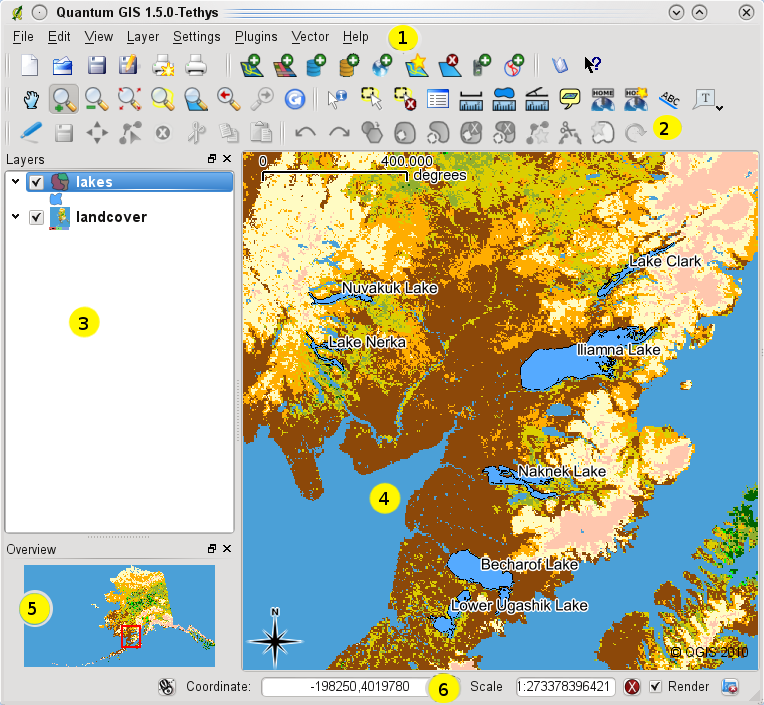
\includegraphics[clip=true, width=12cm]{startup}
   \caption{Interface de \qg avec les données d'essai de l'Alaska \nixcaption\\
   Les numéros cerclés de jaune renvoient aux zones définies dans le texte.}
   \label{fig:startup}
\end{center} 
\end{figure}

\textbf{Note:} Les décorations de fenêtre peuvent vous apparaître différemment sur votre système en fonction de votre système d'exploitation et de votre gestionnaire de fenêtre. \\

L'interface est divisée en 6 zones distinctes :
\begin{center}
\begin{tabular}{p{5cm} p{5cm}}
1. Barre de Menu & 4. Affichage de la carte\\
2. Barre d'Outils & 5. Aperçu de la carte  \\
3. Légende de la carte & 6. Barre de statut \\  
\end{tabular}
\end{center}

Ces 6 composants sont décrits dans les sections suivantes.

\subsection{Barre de Menu}\label{label_menubar}
\index{menus}

La barre de menu fournit un accès aux différentes fonctionnalités de \qg par le biais de menus hiérarchiques. Le menu supérieur et un résumé de certaines options sont listés ci-dessous, avec les icônes des outils correspondants dans la barre d'outils et leurs raccourcis clavier.\footnote{Les raccourcis clavier peuvent maintenant être configurés manuellement (les raccourcis présentés dans cette section sont ceux par défaut) en utilisant l'outil Configurer les Raccourcis dans le menu Préférences.} Bien que les options de menu aient des outils qui leur correspondent et vice-versa, les menus ne sont pas organisés comme les barres d'outils. La barre contenant l'outil est affichée à la suite de chaque option de menu. Pour plus d'informations sur les outils et les barres d'outils, veuillez lire la section \ref{label_toolbars}.

{\setlength{\extrarowheight}{10pt}
\small
\begin{longtable}{p{6cm} p{2cm} p{2.5cm} p{2.5cm}}
Option de menu&Raccourci&Référence&Barre d'outils\\
\endfirsthead
Option de menu&Raccourci&Référence&Barre d'outils\\
\endhead
\multicolumn{4}{r}{Fichier}\\
\dropmenuopttwo{mActionFileNew}{Nouveau Projet}&\keystroke{Ctrl+N}&voir Section \ref{sec:projects}&\dropmenucheck{Fichier}\\
\dropmenuopttwo{mActionFileOpen}{Ouvrir le projet}&\keystroke{Ctrl+O}&voir Section \ref{sec:projects}&\dropmenucheck{Fichier}\\
\dropmenuopt{Ouvrir un projet récent}& &voir Section \ref{sec:projects}&\\
\dropmenuopttwo{mActionFileSave}{Sauvegarder le projet}&\keystroke{Ctrl+S}&voir Section \ref{sec:projects}&\dropmenucheck{Fichier}\\
\dropmenuopttwo{mActionFileSaveAs}{Sauvegarder le projet sous}& \keystroke{Ctrl+Shift+S}&voir Section \ref{sec:projects}&\dropmenucheck{Fichier}\\
\dropmenuopttwo{mActionSaveMapAsImage}{Sauvegarder comme Image}&&voir Section \ref{sec:output}&\\
\dropmenuopttwo{mActionFilePrint}{Paramétrage de l'impression}& \keystroke{Ctrl+P}& voir Section \ref{label_printcomposer}&\dropmenucheck{Fichier}\\
\dropmenuopttwo{mActionFileExit}{Quitter}& \keystroke{Ctrl+Q}&&\\
&&&\\
\multicolumn{4}{r}{Éditer}\\
\dropmenuopttwo{mActionUndo}{Undo}&\keystroke{Ctrl+Z}&voir Section \ref{sec:edit_existing_layer}&\dropmenucheck{Digitizing}\\
\dropmenuopttwo{mActionRedo}{Redo}&\keystroke{Ctrl+Shift+Z}& voir Section \ref{sec:edit_existing_layer}&\dropmenucheck{Digitizing}\\
\dropmenuopttwo{mActionEditCut}{Couper Entités}& \keystroke{Ctrl+X}& voir Section \ref{sec:edit_existing_layer}& \dropmenucheck{Numérisation}\\
\dropmenuopttwo{mActionEditCopy}{Copier Entités}& \keystroke{Ctrl+C}&voir Section \ref{sec:edit_existing_layer} &\dropmenucheck{Numérisation}\\
\dropmenuopttwo{mActionEditPaste}{Coller Entités}& \keystroke{Ctrl+V}&voir Section \ref{sec:edit_existing_layer}&\dropmenucheck{Numérisation}\\
\dropmenuopttwo{mActionCapturePoint}{Capturer le point}&\keystroke{.}&voir Section \ref{sec:edit_existing_layer}& \dropmenucheck{Numérisation}\\
\dropmenuopttwo{mActionCaptureLine}{Capturer la Ligne}& \keystroke{/}& voir Section \ref{sec:edit_existing_layer}& \dropmenucheck{Numérisation}\\
\dropmenuopttwo{mActionCapturePolygon}{Capturer le Polygone}&\keystroke{Ctrl+/}&voir Section \ref{sec:edit_existing_layer}&\dropmenucheck{Numérisation}\\
Et les autres objets du menu d'édition&& voir Section \ref{sec:edit_existing_layer} & \dropmenucheck{Numérisation}\\
\dropmenuopt{Deplacer l'entité}&&&\dropmenucheck{Éditer}\\
\dropmenuopt{Couper entité}&&&\dropmenucheck{Éditer}\\
\dropmenuopt{Effacer la selection}&&&\dropmenucheck{Éditer}\\
\dropmenuopt{Ajouter un sommet}&&&\dropmenucheck{Éditer}\\
\dropmenuopt{Déplacer un sommet}&&&\dropmenucheck{Éditer}\\
\dropmenuopt{Effacer un sommet}&&& \dropmenucheck{Éditer}\\
\dropmenuopt{Ajouter Anneau}\footnote{Nouveauté depuis la version 0.9}&&& \dropmenucheck{Éditer}\\
\dropmenuopt{Ajouter Île}\footnotemark[\value{footnote}] &&&\dropmenucheck{Éditer}\\
&&&\\
\multicolumn{4}{r}{Vue}\\
\dropmenuopttwo{mActionPan}{Se déplacer dans la carte}&&&\dropmenucheck{Navigation}\\
\dropmenuopttwo{mActionZoomIn}{Zoom +}&\keystroke{Ctrl++}&&\dropmenucheck{Navigation}\\
\dropmenuopttwo{mActionZoomOut}{Zoom -}& \keystroke{Ctrl+-}&&\dropmenucheck{Navigation}\\
\dropmenuopttwo{mActionSelect}{Selectionner les entités}&&&\dropmenucheck{Attributs}\\
\dropmenuopttwo{mActionIdentify}{Identifier les données}&\keystroke{I}&&\dropmenucheck{Attributs}\\
\dropmenuopttwo{mActionMeasure}{Mesurer une Ligne}&\keystroke{M}&&\dropmenucheck{Attributs}\\
\dropmenuopttwo{mActionMeasureArea}{Mesurer une Aire}&\keystroke{J}&&\dropmenucheck{Attributs}\\
\dropmenuopttwo{mActionOpenTable}{Zoom Full}& \keystroke{F}&&\dropmenucheck{Navigation}\\
\dropmenuopttwo{mActionZoomToLayer}{Zoom sur l'étendue}&&& \dropmenucheck{Navigation}\\
\dropmenuopttwo{mActionZoomToSelected}{Zoom sur la sélection}&\keystroke{Ctrl+J}&&\dropmenucheck{Navigation}\\
\dropmenuopttwo{mActionZoomLast}{Zoom precédent}&&&\dropmenucheck{Navigation}\\
\dropmenuopt{Zoom taille réelle}&&&\\
\dropmenuopttwo{mActionMapTips}{Infobulles}&&&\dropmenucheck{Attributes}\\
\dropmenuopttwo{mActionNewBookmark}{Nouveau signet}& \keystroke{Ctrl+B}&voir Section \ref{sec:bookmarks} &\dropmenucheck{Attributes}\\
\dropmenuopttwo{mActionShowBookmarks}{Montrer les signets}& \keystroke{B}&voir Section \ref{sec:bookmarks}& \dropmenucheck{Attributes}\\
\dropmenuopttwo{mActionDraw}{Rafraîchir}&\keystroke{Ctrl+R}&&\dropmenucheck{Navigation}\\
&&&\\
\multicolumn{4}{r}{Couche}\\
\dropmenuopttwo{mActionNewVectorLayer}{Nouvelle couche vecteur}&\keystroke{N}& voir Section \ref{sec:create shape}& \dropmenucheck{\scriptsize Gestion des couches}\\
\dropmenuopttwo{mActionAddNonDbLayer}{Ajouter une couche vecteur}& \keystroke{V}&voir Section \ref{label_workingvector}&\dropmenucheck{Fichier}\\
\dropmenuopttwo{mActionAddRasterLayer}{Ajouter une couche raster}& \keystroke{R}&voir Section \ref{label_raster}&\dropmenucheck{Fichier}\\
\dropmenuopttwo{mActionAddLayer}{Ajouter une couche PostGIS}&\keystroke{D}&voir Section \ref{label_postgis}& \dropmenucheck{Fichier}\\
\dropmenuopttwo{mActionAddWmsLayer}{Ajouter une couche WMS}          &\keystroke{W}&voir Section \ref{sec:ogc-wms}& \dropmenucheck{Fichier}\\
\dropmenuopttwo{mActionOpenTable}{Ouvrir la table d'attributs}&&&\dropmenucheck{Attributs}\\
\dropmenuopttwo{mActionToggleEditing}{Activer le mode d'édition}&&&\dropmenucheck{Numérisation}\\
\dropmenuopt{Enregistrer comme Shapefile}&&&\\
\dropmenuopt{Sauvegarder la sélection comme Shapefile}&&&\\
\dropmenuopttwo{mActionRemoveLayer}{Supprimer la couche}& \keystroke{Ctrl+D}&&\dropmenucheck{\scriptsize Gestion des couches}\\
\dropmenuopt{Propriétés}&&&\\
\dropmenuopttwo{mActionInOverview}{Ajouter dans l'aperçu}&&&\keystroke{O}\\
 \dropmenucheck{\scriptsize Gestion des couches}&&&\\
\dropmenuopttwo{mActionAddAllToOverview}{Ajouter tout dans l'aperçu}&\keystroke{+}&&\\
\dropmenuopttwo{mActionRemoveAllFromOverview}{Effacer tout de l'aperçu}&\keystroke{-}&&\\
\dropmenuopttwo{mActionHideAllLayers}{Cacher toutes les couches}&\keystroke{H}&& \dropmenucheck{\scriptsize Gestion des couches}\\
\dropmenuopttwo{mActionShowAllLayers}{Afficher toutes les couches}&\keystroke{S}&&\dropmenucheck{\scriptsize Gestion des couches}\\
&&&\\
\multicolumn{4}{r}{Preférences}\\
\dropmenuopt{Onglets}&&&\\
\dropmenuopt{Barres d'outils}&&&\\
\dropmenuopt{Basculer en mode plein écran}  &&&\\
\dropmenuopttwo{mActionProjectProperties}{Propriétés du projet}&\keystroke{P}&voir Section \ref{sec:projects}&\\
\dropmenuopttwo{mActionCustomProjection}{Projection personnalisée}&&voir Section \ref{sec:customprojections}&\\
\dropmenuopttwo{mActionOptions}{Options} &&voir Section \ref{subsec:gui_options}&\\
&&&\\
\multicolumn{4}{r}{Plugins — (D'autres éléments sont rajoutés en fonction des extensions installées)}\\
\dropmenuopttwo{mActionShowPluginManager}{Gestionnaire d'extension} &&voir Section\ref{sec:managing_plugins}&\dropmenucheck{Extensions}\\
&&&\\
\multicolumn{4}{r}{Aide}\\
\dropmenuopttwo{mActionHelpContents}{Table des matières de l'aide}&\keystroke{F1}&&\dropmenucheck{Help}\\
\dropmenuopttwo{mActionQgisHomePage}{Site officiel de \qg}&&&\\\keystroke{Ctrl+H}
\dropmenuopttwo{mActionCheckQgisVersion}{vérifier la version \qg}&&&\\
\dropmenuopttwo{mActionHelpAbout}{A propos}&&&\\
\end{longtable}}

\subsection{Barre d'outils}\label{label_toolbars}
\index{toolbars}

La barre d'outils fournit un accès à la majorité des fonctions des menus en plus d'outils additionnels destinés à interagir avec la carte. Chaque outil dispose d'une bulle d'aide qui s'affiche lorsque vous placez votre curseur au-dessus, elle affiche une courte description de son rôle.

Chaque barre de menu peut être déplacée selon vos besoins. Vous pouvez les désactiver en utilisant le bouton droit de votre souris en survolant la barre de menu.

\begin{Tip}
\caption{\textsc{Restaurer la barre d'outil}} \index{layout!toolbars}
Si vous avez accidentellement masqué toutes vos barres d'outils, vous pouvez les récupérer en sélectionnant \mainmenuopt{Paramétrage} > \dropmenuopt{Barre d'outils}.
\end{Tip}

\subsection{Légende cartographique}\label{label_legend}
\index{legend}

La zone de légende cartographique est utilisée pour définir la visibilité et l'ordre d'empilement des couches. Une couche se situant au sommet de la liste de cette légende sera affichée au-dessus de celles qui se situent plus bas dans la liste. La boîte présente à côté de chacune des couches permet d'afficher ou de cacher.\index{layer!visibility}

Les couches peuvent être rassemblées en créant un groupe et en y glissant les couches désirées. Pour ce faire, déplacez votre curseur sur la légende, faites un clic droit puis choisissez \dropmenuopt{Ajouter un groupe}. Un nouveau dossier est apparu, vous pouvez maintenant glisser et déposer les couches sur le symbole de ce dossier. Il est possible de basculer le mode d'affichage de toutes les couches d'un groupe en décochant seulement le groupe. Pour retirer une couche d'un groupe, il suffit de pointer votre curseur sur elle, de faire un clic droit et de choisir \dropmenuopt{Mette l'item au-dessus}. Pour changer le nom du groupe sélectionnez \dropmenuopt{Renommer} dans le menu contextuel du groupe.

Le contenu du menu contextuel affiché par un clic droit varie si la couche sélectionnée est un raster ou un vecteur. Pour les couches vectorielles GRASS \dropmenuopt{Basculer en mode édition} n'est pas disponible. Veulliez lire la section \ref{grass_digitising} pour plus d'informations sur l'édition de couches vecteurs GRASS.

\begin{itemize}[label=--]
\item \textbf{Menu clic droit pour les couches raster}
\begin{itemize}[label=--]
\item \dropmenuopt{Zoomer sur l'emprise de la couche}
\item \dropmenuopt{Zoomer à la meilleure échelle (100\%)}
\item \dropmenuopt{Montrer dans l'aperçu}
\item \dropmenuopt{Effacer}
\item \dropmenuopt{Propriétés}
\item \dropmenuopt{Renommer}
\item \dropmenuopt{Ajouter un groupe}
\item \dropmenuopt{Etendre tout}
\item \dropmenuopt{Réduire tout}
\item \dropmenuopt{Montrer les groupes de fichiers}
\end{itemize}

\item \textbf{Menu clic droit pour les couches vecteurs}
\begin{itemize}[label=--]
\item \dropmenuopt{Zoomer sur l'emprise de la couche}
\item \dropmenuopt{Montrer dans l'aperçu}
\item \dropmenuopt{Effacer}
\item \dropmenuopt{Ouvrir la table d'attributs}
\item \dropmenuopt{Basculer en mode édition}
\item \dropmenuopt{Sauvegarder comme shapefile}
\item \dropmenuopt{Enregistrer la sélection comme shapefile}
\item \dropmenuopt{Propriétés}
\item \dropmenuopt{Mettre l'item au-dessus}
\item \dropmenuopt{Renommer}
\item \dropmenuopt{Ajouter un groupe}
\item \dropmenuopt{Etendre tout}
\item \dropmenuopt{Réduire tout}
\item \dropmenuopt{Montrer les groupes de fichiers}
\end{itemize}

\item \textbf{Menu clic droit pour les groupes} 
\begin{itemize}[label=--]
\item \dropmenuopt{Effacer}
\item \dropmenuopt{Renommer}
\item \dropmenuopt{Ajouter un groupe}
\item \dropmenuopt{Etendre tout}
\item \dropmenuopt{Réduire tout}
\item \dropmenuopt{Montrer les groupes de fichiers}
\end{itemize}

\end{itemize}

Si plusieurs sources de données vecteurs ont le même type de vecteur (points, lignes ou polygones) et les mêmes attributs, leurs représentations peuvent être groupées. Cela signifie que si la représentation d'une couche est modifiée, toutes les autres en bénéficieront automatiquement. Pour grouper la symbologie, faites un clic droit dans la zone de légende et sélectionnez \dropmenuopt{Montrer les groupes de fichiers}. Les groupes de fichiers relatifs aux couches apparaissent, il est maintenant possible de déplacer un fichier d'un groupe à un autre. Si vous le faites, les fichiers seront regroupés. Notez que \qg le permet seulement si les 2 couches sont susceptibles de partager le même type de symbologie.

\subsection{Vue de la carte}\label{label_mapview}
\index{map!view} 

C'est la partie centrale de \qg — les cartes sont affichées dans cette partie ! Celle qui s'affiche dépend des couches raster et vecteurs que vous avez choisi de charger (lire les sections suivantes pour savoir comment charger une couche). La vue de la carte peut être modifiée en portant le focus sur une autre région, ou en zoomant en avant ou en arrière. Plusieurs opérations peuvent être effectuées sur la carte comme il est expliqué dans les descriptions des barres d'outils. La vue de la carte et la légende sont étroitement liées — la carte reflète les changements que vous opérez dans la légende.

\begin{Tip}\caption{\textsc{Zoomer la carte avec la molette de la souris}\index{zoom!mouse wheel}}
Vouspouvez utiliser la molette de la souris pour changer le niveau de zoom de la carte. Placez votre curseur dans la zone d'affichage de la carte et faites rouler la molette vers l'avant pour agrandir et faites là rouler vers vous pour zoomer en arrière. La position du curseur est le centre sur lequel va s'opérer le zoom. Vous pouvez modifier le comportement du zoom de la souris en utilisant l'onglet \tab{Outils cartographiques} dans le menu \mainmenuopt{Paramètres} >\dropmenuopt{Options}.
\end{Tip}

\begin{Tip}\caption{\textsc{Déplacer la carte avec les flèches et la barre espace}}\index{pan!arrow keys}
Vous pouvez utiliser les flèches du clavier pour se déplacer sur la carte? Placez le curseur sur la carte et appuyez sur la flèche droite pour vous diriger vers l'Est, la flèche gauche pour aller vers l'Ouest, la flèche supérieure pour le Nord et la flèche inférieure pour le Sud. Vous pouvez aussi déplacer la carte en gardant la touche espace appuyée et en bougeant la souris.
\end{Tip}

\subsection{Aperçu de la carte}\label{label_mapoverview}
\index{map!overview}

La zone d'aperçu de la carte permet d'avoir une vue totale de l'emprise des couches ajoutées au projet, elle peut être sélectionnée dans le menu\mainmenuopt{Préférences} >\dropmenuopt{Panneaux}. Au sein de cette fenêtre se situe un rectangle qui représente l'étendue de la carte, cela permet de savoir quelle région de la carte vous êtes en train de visualiser. Les étiquettes ne sont pas affichées dans l'aperçu même si les couches visibles ont l'affichage de leurs étiquettes activées.
Vous pouvez rajouter une couche dans l'aperçu en faisant un clic-droit dessus dans la légende ou en sélectionnant \checkbox{Montrer dans l'aperçu}. Vous pouvez aussi rajouter des couches ou en ôter de l'aperçu en utilisant les outils d'aperçu dans la barre d'outils.

Si vous cliquez et déplacez le rectangle rouge qui montre votre emprise actuelle, la vue principale se mettra en conséquence.

\subsection{Barre de statuts}\label{label_statusbar}

La barre de statuts montre votre position dans les coordonnées de la carte (p. ex. mètres ou degrés décimaux) lorsque vous déplacez votre curseur. À gauche de l'affichage des coordonnées se trouve un petit bouton qui bascule entre les coordonnées de la position ou l'étendue de la zone que vous visualisez.

Une barre de progression dans la barre de statuts vous montre le cheminement du rendu au fur et à mesure qu'une couche est dessinée sur l'écran. Dans certains cas, tel que lors de l'établissement de statistiques d'une couche raster, la barre indique le statut des opérations qui prennent du temps.

Si une nouvelle extension ou une mise à jour est disponible, vous verrez un message dans la barre de statut. Sur la droite, une boîte à cocher peut être utilisée pour bloquer le rendu des couches sur la carte (voir Section \ref{subsec:redraw_events}). A l'extrémité se situe l'icône de projection,  un clic dessus ouvrira la fenêtre de propriétés de projection pour le projet en cours.

\begin{Tip}\caption{\textsc{Calculer l'échelle correcte de la vue de la carte}}\index{scale!calculate}
Quand vous démarrez \qg, les degrés sont l'unité par défaut et indique à \qg que toutes les coordonnées de votre couche sont en degrés. Pour avoir les valeurs correctes de l'échelle, vous pouvez soit passer en mètre manuellement avec l'onglet \tab{Gééral} sous le menu \mainmenuopt{Préférences} >\dropmenuopt{Propriétés du projet} ou vous pouvez sélectionner un système de projection de référence en cliquant sur \toolbtntwo{mIconProjectionDisabled}{projection}. Dans ce dernier cas, les unités sont automatiquement choisies selon les spécifications de la projection, p. ex. '+units=m'.
\end{Tip}

\section{Rendu}\label{subsec:redraw_events}\index{rendering}

Par défaut, \qg effectue le rendu de toutes les couches visibles à chaque fois que l'affichage de la carte a besoin d'être mise à jour. Les événements qui déclenchent ce rafraîchissement incluent :

\begin{itemize}[label=--]
\item L'ajout d'une couche
\item Un déplacement ou un zoom
\item Un redimensionnement de la fenêtre de \qg
\item Un changement de la visibilité d'une couche
\end{itemize}

\subsection{Rendu dépendant de l'échelle}\index{rendering!scale dependent}
\label{label_scaledepend}

Le rendu dépendant de l'échelle permet de spécifier l'échelle minimale et maximale à laquelle la couche doit être visible. Pour définir une échelle de rendu, ouvrez la fenêtre de \dialog{Propriétées} en double-cliquant sur une couche dans la légende et dans l'onglet \tab{Général}, saisissez les valeurs voulues et cocher la case \checkbox{Utiliser le rendu dépendant de la mise à l'échelle}.

Vous pouvez déterminer les valeurs d'échelle en zoomant au niveau que vous voulez utiliser et en notant les valeurs de la barre d'état.\index{scale}

\subsection{Contrôler le rendu}\label{label_controlmap}

Le rendu de la carte peut être contrôlé de différentes manières :

\minisec{a) Suspendre le rendu}\index{rendering!suspending}
\label{label_suspendrender}

Pour suspendre le rendu, cliquez sur la case \checkbox{Rendu}dans le coin inférieur droit de la barre de statut. Quand cette case n'est pas coché, \qg ne redessine pas la carte en réponse aux événements décrits dans la section \ref{subsec:redraw_events}. Voici quelques cas pour lequel vous pourriez vouloir le faire :

\begin{itemize}[label=--]
\item Ajouter beaucoup de couches et les symboliser avant d'effectuer un rendu potentiellement long
\item Ajouter une ou plusieurs couches et définir une échelle
\item Ajouter une ou plusieurs couches et et zoomer sur un endroit spécifique
\item N'importe quelle combinaison des éléments précédents
\end{itemize}

Cocher la case \checkbox{Rendu} activera de nouveau le rendu et provoquera un rafraîchissement immédiat de la vue active.

\minisec{b) Définir les options d'ajout de couche}\label{label_settinglayer}
\index{rendering!options}\index{layers!initial visibility}

Il est possible de définir une option qui chargera toutes les nouvelles couches sans les dessiner, elles seront ajoutées à la carte, mais la case de visibilité sera décochée par défaut. Pour définir cette option, sélectionnez l'option \mainmenuopt{Préférences} > \dropmenuopt{Options} et cliquez sur l'onglet \tab{Rendu}. Décochez la case \checkbox{par défaut les couches supplémentaires sont affichées}. Les nouvelles couches ajoutées à la carte seront invisibles par défaut.

\minisec{Arrêter le rendu}\index{rendering!halting}
\label{label_stoprender}

Pour arrêter le rendu de la carte, appuyez sur la touche ESC. Ceci stoppera le rafraîchissement de la vue de la carte et laissera la carte partiellement dessinée. Il est possible qu'il y ait un délai entre le moment où la touche est pressée et le temps que le rendu de la carte soit arrêté.

\textbf{NOTE}: Il n'est pas actuellement possible d'arrêter le rendu de cette manière — ça été désactivé avec le port qt4 du fait d'instabilités.

\minisec{c) Mettre à jour l'affichage de la carte pendant le rendu}
\label{label_updatemap}\index{rendering!update during drawing}

Vous pouvez définir une option pour mettre à jour l'affichage de la carte quand des entités sont dessinées. Par défaut, \qg n'affiche pas les entités d'une couche tant que la couche entière n'a pas été rendue. Pour mettre à jour l'affichage à mesure que les entités sont lues dans la table attributaire, sélectionnez le menu \mainmenuopt{Settings} > \dropmenuopt{Options} puis l'onglet \tab{Rendu}. Mettez comme valeur le nombre d'entités à mettre à jour durant le rendu. Si elle est égale à 0, cela désactive la mise à jour durant le dessin (c'est la valeur par défaut). Une valeur trop basse risque d'impacter les performances, car la vue de la carte sera constamment mise à jour durant la lecture des entités. Il est suggéré de commencer à 500.

\minisec{d) Influencer la qualité du rendu}
\label{label_renderquality}\index{rendering!quality}

Pour influencer la qualité du rendu de la carte vous avez trois possibilités. Dans le menu \mainmenuopt{Préférences} > \dropmenuopt{Options} puis l'onglet \tab{Rendu} et sélectionnez/désélectionnez les cases suivantes :
\begin{itemize}[label=--]
\item \checkbox{Les lignes semblent moins déchiquetées aux dépens d'une certaine vitesse d'exécution}
\item \checkbox{Corriger les polygones remplis de manière erronée}
%\item \checkbox{Rafraîchir en permanence lors du déplacement de la table des matières/carte}
\end{itemize}

\section{Mesurer}\label{sec:measure}\index{measure}

Les mesures fonctionnent uniquement au sein des systèmes de coordonnées projetées (exemple : UTM, Lambert 93). SI la couche active est définie par système géographique de coordonnée (latitude/longitude), les résultats d'une mesure de ligne ou d'aires seront incorrects. Pour y remédier, vous devez mettre un système de coordonnées approprié (voir Section~\ref{label_projections}).

\subsection{Mesurer une longueur et une aire}\index{measure:line length}\index{measure:areas}
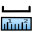
\includegraphics[width=0.7cm]{mActionMeasure} 
\qg peut mesurer des distances réelles entre plusieurs points selon un ellipsoïde défini. Pour le configurer, allez dans le menu \mainmenuopt{Préférences} > \dropmenuopt{Options}puis dans l'onglet \tab{Outils cartographiques} et choisissez l'ellipsoïde approprié. Vous pouvez également modifier ici l'unité de mesure (mètre ou pied). Cet outil permet de placer des points sur la carte. Chaque longueur de segment s'affiche dans la fenêtre de mesure avec la longueur additionnée totale. Pour stopper les mesures, faites un clic droit. \par
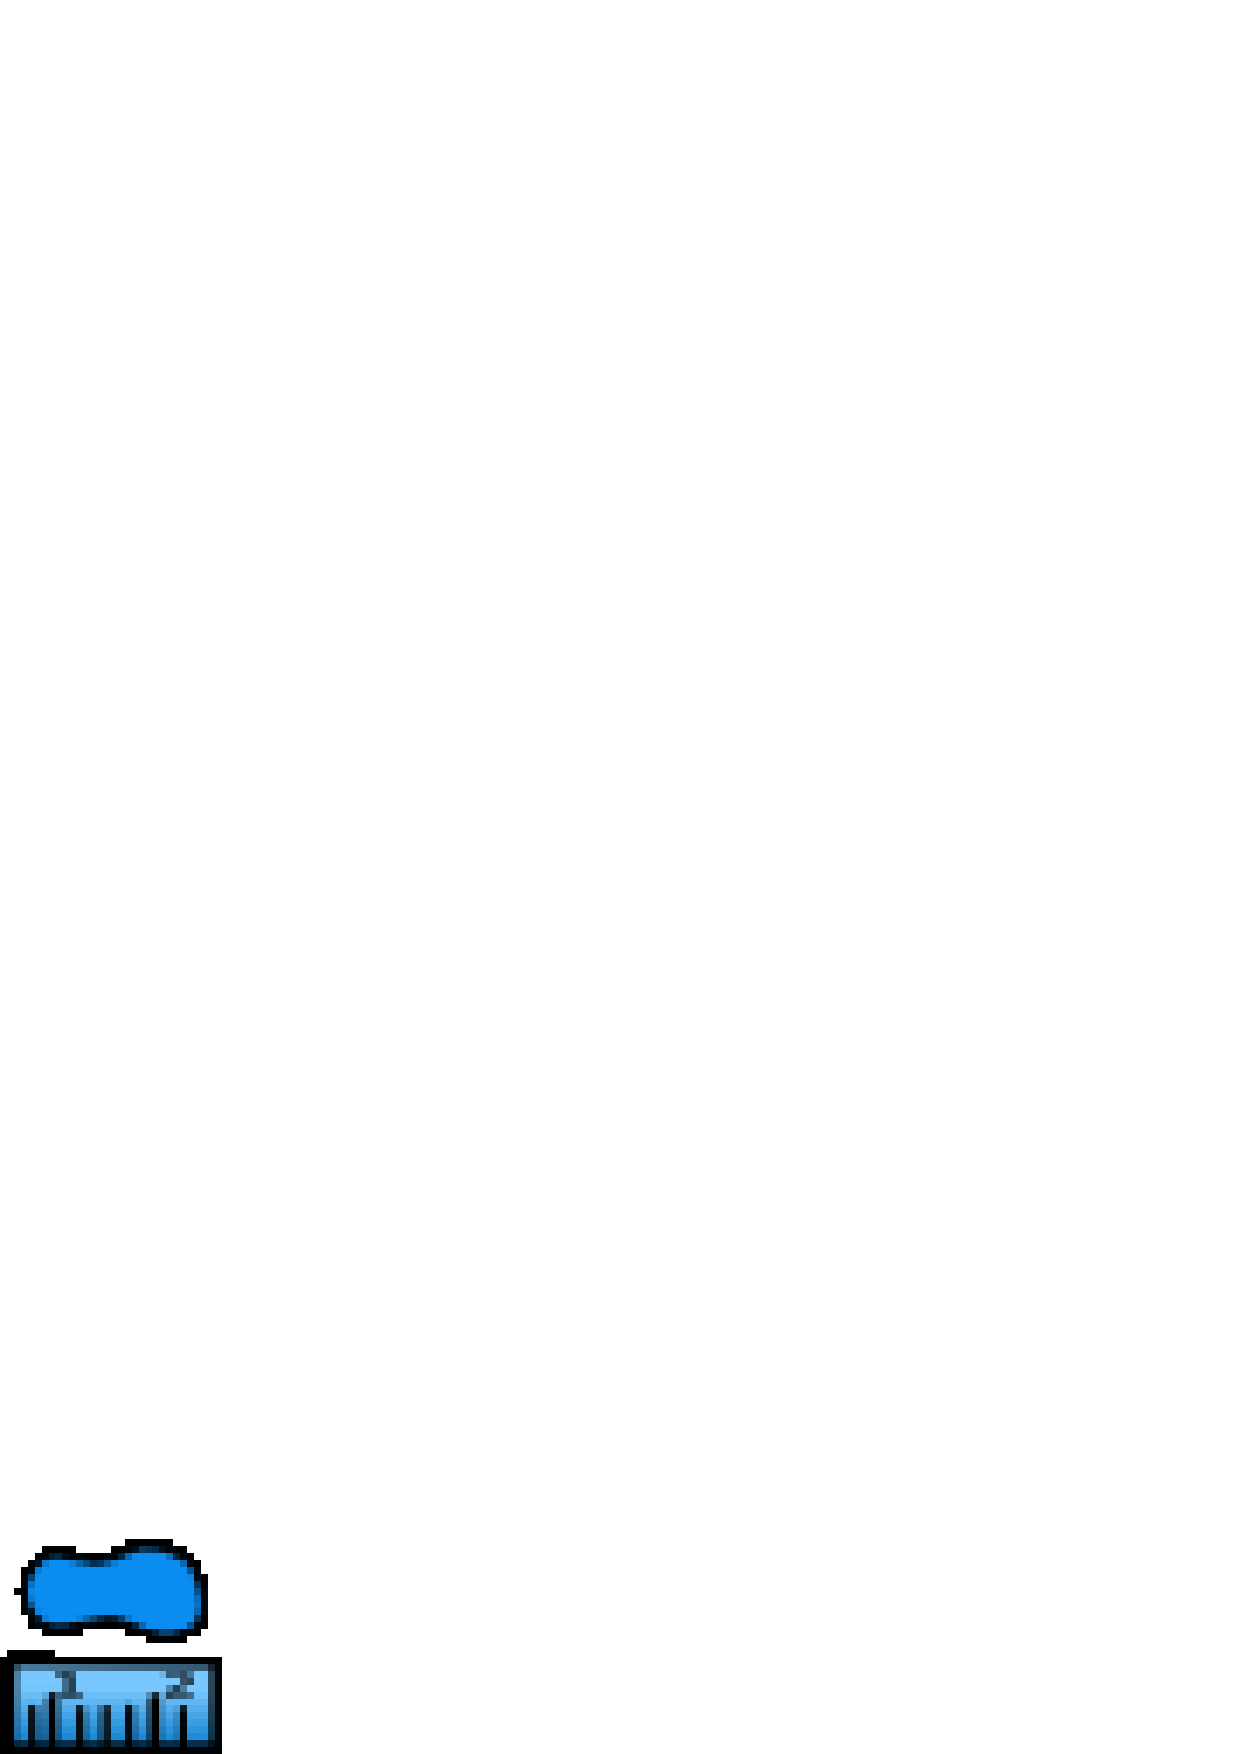
\includegraphics[width=0.7cm]{mActionMeasureArea} Les aires peuvent aussi être mesurées.
Dans la fenêtre de mesure apparaît la surface totale mesurée. \par
En complément, l'outil de mesure s'accrochera à la couche sélectionnée à partir du moment où celle-ci à un seuil d'accrochage défini (voir la section \ref{snapping_tolerance}). Donc si vous voulez mesurez avec exactitude une ligne ou le contour d'un polygone, spécifiez d'abord un seuil d'accrochage puis avec l'outil de mesure chaque clic de souris se situant dans ce seuil s'accrochera aux entités de cette couche.

\begin{figure}[ht]
\centering
  \subfloat[Mesure de lignes] {\label{subfig:measure_line}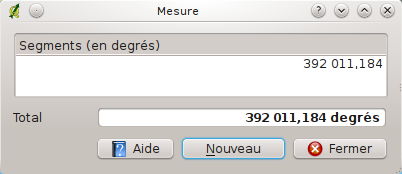
\includegraphics[clip=true, width=0.3\textwidth]{measure_line}}
  \hspace{1cm}
  \subfloat[Mesure d'aires]{\label{subfig:measure_area}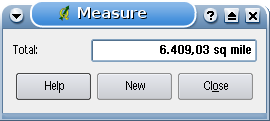
\includegraphics[clip=true, width=0.3\textwidth]{measure_area}}
  \caption{Outils de mesure \nixcaption} \label{fig:measure}
\end{figure}

\section{les projets}\label{sec:projects}\index{projets}

L'état de votre session de \qg est considéré comme étant un projet. \qg ne peut travailler que sur un projet à la fois. Les propriétés sont considérées comme étant assignées à un projet ou comme étant par défaut pour les nouveaux projets ( voir Section \ref{subsec:gui_options}). \qg peut enregistrer l'état de votre travail dans un fichier de projet en utilisant le menu the state of your 
workspace into a project file using the menu options 
\mainmenuopt{Fichier} > \dropmenuopttwo{mActionFileSave}{Sauvegarder le projet}
ou \mainmenuopt{Fichier} > \dropmenuopttwo{mActionFileSaveAs}{Sauvegarder le projet sous...}.

Pour charger un projet dans une session \qg, aller dans \mainmenuopt{Fichier} > \dropmenuopttwo{mActionFileOpen}{Ouvrir un Projet} ou \mainmenuopt{Fichier} > \dropmenuopt{Ouvrir un projet récent}. Si vous souhaitez revenir à une session vierge, aller sur \mainmenuopt{Fichier} > \dropmenuopttwo{mActionFileNew}{Nouveau Projet}.
Chacune de ces options vous demandera si vous désirez enregistrer le projet si des changements ont été effectués depuis son ouverture ou sa dernière sauvegarde.

Les types d'informations enregistrées dans un projet sont :

\begin{itemize}[label=--]
\item Les couches ajoutées
\item Les propriétés des couches ainsi que de symbologie
\item La projection de la carte
\item L'étendue de la dernière zone de visualisation
\end{itemize}

Le fichier de projet est enregistré au format XML, il est donc possible de l'éditer en dehors de \qg si vous savez ce que vous faites. Le format a été modifié à plusieurs reprises depuis les versions antérieures de \qg, les fichiers enregistrés sous ces dernières peuvent ne plus fonctionner correctement. Pour être averti dans genre de cas, allez dans l'onglet \tab{Général} du menu \mainmenuopt{Préférences} > \dropmenuopt{Options} et sélectionnez\\ \checkbox{\small M'avertir lors de l'ouverture d'un fichier projet sauvegardé avec une version précédente de \qg}.

\minisec{Propriétés de projet}
Dans la fenêtre de propriétés du projet vous pouvez mettre des options spécifiques à un projet. Cela inclut :
\begin{itemize}[label=--]
 \item Dans l'onglet \tab{Général} le titre du projet, les unités, et la possibilité d'enregister des chemins relatifs vers les couches. L'édtion topologique et les options d'accrochage peuvent être changés ici.
\item L'onglet \tab{Système de Coordonnées de Référence (SCR)} permet de choisir le système de coordonnées pour ce projet et d'activer la projection à la volée des couches vecteurs utilisants un SCR différent.
\item Avec le troisième onglet \tab{Identification des couches} vous pouvez activer (ou désactiver) les couches qui répondront à l'outil d'identification (voir le paragraphe sur les outils de la carte dans la section \ref{subsec:gui_options})
\end{itemize}

\section{Sauvegarder l'affichage}\label{sec:output}\index{output!save as image!print composer!quick print}
Il y a plusieurs façons d'enregistrer un fichier depuis votre session. Nous en avons déjà vu une dans la section \ref{sec:projects} : sauvegarder dans un fichier de projet.
Voici d'autres manières de procéder à l'enregistrement de fichiers :
\begin{itemize}[label=--]
\item Menu option \dropmenuopttwo{mActionSaveMapAsImage}{Sauvegarder comme une Image} ouvre une fenêtre de dialogue où vous devez saisir le nom, le chemin et le type d'images (PNG ou JPEG). Depuis la version 1.1.0, un fichier "world" avec une extension PNGW ou JPGW est enregistré dans le même dossier que l'image géoréférencée.
\item Menu option \dropmenuopttwo{mActionFilePrint}{Paramètrage de l'impression} ouvre une fenêtre de dialogue où vous pouvez faire une mise en page et imprimer la vue active de la carte (voir Section~\ref{label_printcomposer})
\end{itemize}

\section{Options d'affichage}\label{subsec:gui_options}

\includegraphics[width=0.7cm,clip=true]{mActionOptions} 
Quelques options basiques peuvent être sélectionnés en allant dans le menu \mainmenuopt{Préférences} >
\dropmenuopttwo{mActionOptions}{Options}. Les onglets dans lesquels vous pouvez configurer les options sont :

\minisec{Onglet Général}

\begin{itemize}[label=--]
\item \checkbox{Demander à sauvegarder les changements apportés au projet si requis}
\item \checkbox{\small M'avertir lors de l'ouverture d'un fichier projet sauvegardé avec une version précédente de \qg}
\item \checkbox{Changer la couleur de la sélection du fond d'écran}
\item Changer le thème des icônes
\item \checkbox{Mettre les noms de couche en majuscule dans la légende}
\item \checkbox{Afficher les noms des attributs de classifications dans la légende}
\item \checkbox{Cacher l'écran de démarrage}
\item \checkbox{Ouvrir les résultats identifiés dans une fenêtre détachée (redémarrage requis)}
\item \checkbox{Ouvrir la table d'attributs dans une fenêtre mobile}
\item \checkbox{Ajouter une couche PostGIS avec un double-clic et sélectionner en mode étendu}
%\item Définir le comportement de la table d'attributs (choisir entre montrer toutes les entités, celles sélectionnées et celles présentes dans la vue active)
\end{itemize}

\minisec{Onglet de Rendu}

\begin{itemize}[label=--]
\item \checkbox{par défaut les couches supplémentaires sont affichées}
\item Définir le nombre d'entités à dessiner avant d'actualiser l'affichage
\item \checkbox{\small Les lignes semblent moins déchiquetées aux dépens d'une certaine vitesse d'exécution}
\item \checkbox{Corriger les polygones remplis de manière erronée}
%\item \checkbox{Rafraîchir en permanence la table des matières/carte lors du déplacement} 
\end{itemize}

\minisec{Onglet des Outils Cartographiques}

\begin{itemize}[label=--]
\item Spécifier le rayon de recherche comme pourcentage de la largeur de la carte)
\item Définir l'ellipsoïde pour des calculs de distance
\item Définir la couleur de l'étirement pour les outils de mesure
\item Définir l'action de la molette de la souris (Zoomer, Zoomer et récentrer, Zoomer sur le curseur de la souris, Rien)
\item Définir le facteur de zoom
\end{itemize}

\minisec{Revêtement}

\begin{itemize}[label=--]
\item Définir l'algorythme de placement des étiquettes (choisir entre le point central (par défaut), chain, popmusic tabu chain, popmusic tabu et popmusic chain)
\end{itemize}

\minisec{Onglet de Numérisation}

\begin{itemize}[label=--]
\item Définir la couleur et la largeur de la ligne d'étirement
\item Définir le mode d'accrochage par défaut (à un vertex, un segment, aux vertex et segments)
\item Définir la tolérance d'accrochage par défaut (en unités de la couche) 
\item Définir le rayon de recherche pour l'édition des sommets (en unités de la couche)
\item Définir les marqueurs de sommet (croix ou cercle semi-transparent)
\item \checkbox{Montrer les marqueurs seulement pour les entités sélectionnées}
\item \checkbox{Supprimer la fenêtre d'attributs apparaissant après chaque création d'entité}
\end{itemize}

\minisec{Onglet de SCR}

\begin{itemize}[label=--]
\item \checkbox{Demander pour le Système de Coordonnées de Référence (SCR)}
\item \checkbox{La projection globale par défaut du projet qui sera employée}
\item \checkbox{La projection par défaut ci-dessous sera employée}
\item Sélectionner le Système de Coordonnées de Référence (SCR) par défaut
\end{itemize}

\minisec{Onglet de Paramètres du lieu}

\begin{itemize}[label=--]
\item \checkbox{Forcer la nationalité du système}
\item Paramètres de lieu sur votre système
\end{itemize}

\minisec{Onglet Proxy}
{\setlength{\baselineskip}{1.4\baselineskip}
\begin{itemize}[label=--]
\item \checkbox{Utiliser un proxy pour l'accès internet}, définition de l'hôte, du port, de l'utilisateur et du mot de passe.
\item Modifiez le \dropmenuopt{type de Proxy} selon vos besoins
 \begin{itemize}[label=--,itemsep=2pt]
  \item \dropmenuopt{Proxy par défaut}: ce proxy est déterminé en basant sur le proxy de l'application
  \item \dropmenuopt{Socks5Proxy}: proxy générique pour n'importe quel type de connexion. Supporte TCP, UDP, le lien à un port (pour les connexions entrantes) et l'authentication
  \item \dropmenuopt{HttpProxy}: utilise la commande \og CONNECT \fg, supporte seulement les connexions TCP sortantes et l'authentication
  \item \dropmenuopt{HttpCachingProxy}: utilise les commandes normales HTTP, c'est utile uniquement dans le contexte de requête HTTP
  \item \dropmenuopt{FtpCachingProxy}: utilise un proxy FTP, ce n'est utile que dans le cas de requête FTP
\end{itemize}
\end{itemize}}
L'exclusion d'adresses peut être ajoutée dans la boîte de texte en dessous des paramètres de proxy (voir fig. \ref{fig:proxy-settings}) en pressant le bouton \button{Ajouter}. Ensuite double-cliquer sur l'URL nouvellement créée est entrer l'adresse que vous voudriez exclure du proxy. Le bouton \button{Supprimer} efface l'entrée sélectionnée.

Si vous désirez des informations plus détaillées sur les différents paramètres, veuillez vous référer au manuel de la bibliothèque Qt à \url{http://doc.trolltech.com/4.5/qnetworkproxy.html#ProxyType-enum}.

\begin{figure}[ht]
   \begin{center}
   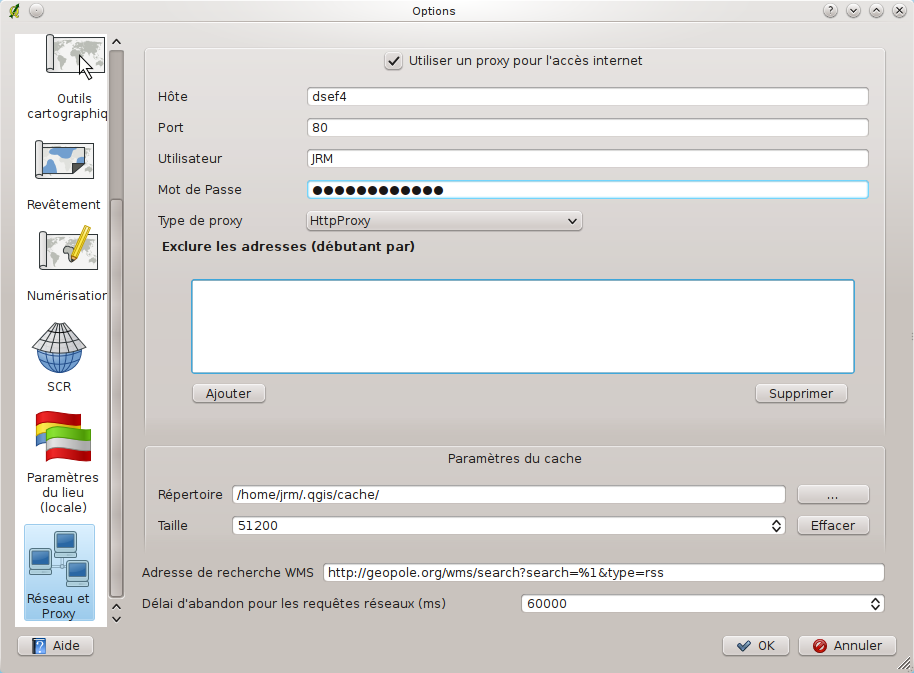
\includegraphics[clip=true, width=10cm]{proxy-settings}
   \caption{Proxy-settings in \qg \nixcaption}
   \label{fig:proxy-settings}
\end{center} 
\end{figure}

\begin{Tip} \caption{\textsc{Utiliser un proxy}}
Utiliser un serveur mandataire (proxy) peut être compliqué, vous pouvez multiplier les essais et erreurs en cochant les cases jusqu'à obtenir une connexion qui vous satisfasse.
\end{Tip}

Vous pouvez modifier ces options selon vos besoins, certains de ces changements nécessiteront un redémarrage avant d'être effectifs.

\begin{itemize}[label=--]
\item \nix{les paramètres sont enregistrés dans un fichier texte:\\ \$HOME/.config/QuantumGIS/qgis.conf}
\item \osx{les paramètres sont enregistrés dans: \$HOME/Library/Preferences/org.qgis.qgis.plist}
\item \win{les paramètres sont enregistrés dans le registre sous:}
\begin{verbatim}
\\HKEY\CURRENT\USER\Software\QuantumGIS\qgis
\end{verbatim}
\end{itemize}

\section{Signets spatiaux}\label{sec:bookmarks}
\index{bookmarks}
\index{spatial bookmarks|\voir{bookmarks}}

Les signets spatiaux vous permettent de marquer une zone de la carte pour y retourner plus tard.

\subsection{Créer un signet}
Pour créer un signet :
\begin{enumerate}
\item Déplacez-vous sur la zone concernée
\item Sélectionnez le menu \mainmenuopt{Vue} > \dropmenuopt{Nouveau signet} ou appuyez sur la touche \keystroke{Ctrl-B}
\item Entrez un nom pour décrire le signet (jusqu'à 255 caractères)
\item Cliquez sur \button{OK} pour ajouter le signet ou sur \button{Annuler} pour sortir de la fenêtre sans l'enregistrer
\end{enumerate}

Vous pouvez avoir plusieurs signets portant le même nom.

\subsection{Travailler avec les signets}
Pour utiliser ou gérer les signets allez dans le menu \mainmenuopt{Vue} > \dropmenuopt{Montrer les signets}.
Le dialogue \dialog{Signets géospatiaux} vous permet de zoomer ou d'effacer un signet.
Vous ne pouvez pas modifier le nom d'un signet ou ses coordonnées.

\subsection{Zoomer sur un signet}
Depuis la fenêtre \dialog{Signets géospatiaux}, sélectionner le signet voulu en cliquant dessus puis sur le bouton \button{Zoomer sur}. Vous pouvez aussi zoomer en opérant un double-clic.

\subsection{Effacer un signet}
Pour effacer un signet depuis la fenêtre \dialog{Signets géospatiaux}, cliquez dessus puis sur le bouton \button{Effacer}.
Confirmez votre choix en cliquant sur \button{Oui} ou annuler en cliquant sur \button{Non}
